\section{Solving Identification with a Selection Model}
\label{sec:selectionmodel}
If your goal is to estimate CM effects, and you could control for unobserved selection terms $U_{0,i}, U_{1,i}$, then you would.
This ideal example would yield unbiased estimates for the ADE and AIE.
% Alas, $U_i$ is by definition unobserved.
A selection model takes this insight seriously, providing conditions to model the implied confounding by $U_{0,i}, U_{1,i}$, and then controlling for it.

The main problem is that second-stage reqression equation \eqref{eqn:parametric-secondstage} is not identified, because $U_{0,i}$ and $U_{1,i}$ are unobserved.
\begin{align*}
    \Egiven{Y_i}{Z_i, D_i, \vec X_i} \;\; =& \;\;
        \alpha
        + \beta D_i
        + \gamma Z_i
        + \delta Z_i D_i
        + \varphi(\vec X_i) \\
        & \;\; +\left( 1 - D_i \right) \Egiven{ U_{0,i} }{D_i = 0, \vec X_i}
            + D_i \Egiven{ U_{1,i} }{D_i = 1, \vec X_i}
\end{align*}
The following assumptions are sufficient to model the correlated error terms, identifying $\beta, \gamma, \delta$, and thus both the ADE and AIE.

\textbf{Needs more story telling of how this happens.}

\textbf{Writing plan:} set up a sequence of assumption X $\implies$ implcation X.
Then a paragraph underneath, explaining what it is doing.
See \cite{kline2019heckits} for an excellent example of this.

Additionally, suppose the vector of control variables $\vec X_i$ has at least two entries;
denote $\vec X_i^{\text{IV}}$ as one entry in the vector, and $\vec X_i^-$ as the remaining rows.
\begin{definition}
    \label{dfn:controlfun-assumptions}
    Control function assumptions.
    \begin{align}
        \label{eqn:firststage-monotonicity}
        &\Probgiven{ D_i(1) \geq D_i(0) }{\vec X_i} = 1 \\
        \label{eqn:controlfun-ident}
        &D_i \indep Y_i(.,.) \; \Big| \; \vec X_i^-, K_i \\
        \label{eqn:controlfun-iv}
        &\vec X_i^{\text{IV}} \textnormal{ satisfies }
        \partialdiff{\vec X_i^{\text{IV}}}\left[
            \mu_1(\vec X_i) - \mu_0(\vec X_i)\right] = 0
            < \partialdiff{\vec X_i^{\text{IV}}}\Egiven{D_i(z')}{\vec X_i},
            \textnormal{ for } z' = 0, 1.
    \end{align}
\end{definition}
Assumption \ref{dfn:controlfun-assumptions}\eqref{eqn:firststage-monotonicity} is the (conditional) monotonicity assumption \citep{imbens1994identification}, which is untestable but acceptable in many empirical applications.
Assumption \ref{dfn:controlfun-assumptions}\eqref{eqn:controlfun-ident} is the control function assumption, assuming that first-stage unobserved heterogeneity explains second-stage selection into $D_i$.
Assumption \ref{dfn:controlfun-assumptions}\eqref{eqn:controlfun-iv} is assuming that an instrument exists, which satisfies an exclusion restriction (i.e., not impacting mediator gains $\mu_1-\mu_0$), and has a non-zero influence on the mediator (i.e., strong first-stage).
The exclusion restriction is untestable, and must be guided by domain-specific knowledge; strength of the first-stage is testable, and must be justified with data by methods common in the instrumental variables literature.


Writing here about how a \cite{heckman1974shadow} selection model purges selection bias.



Control function assumption + instrument.

Lemma: Under assumptions CF(1, 2, 3), mean POs are identified in the way written in Kline Walters (2019).
Needs an appendix proof.

This is exploiting ideas from selection models + marginal TEs to identify this system, including using the selection model to identify the mediator compilers’ effect.  Indeed, mediation estimates already do a two-step procedure; it is a minor adjustment to include a CF  in the second-stage, to guard against selection-on-gains (chief among which is the Roy model).

Monotonicity gives selection model representation, $D = 1{ \phi(Z, X) > V }$ which can be transformed into $D = 1{ \pi(Z, X) > U }$ for $U_i = F_V(V_i) ~ unif(0, 1)$.
CF assumption connects first-stage and second-stage errors, by assuming that $Cov(U_i, U_1),Cov(U_i, U_0)  > 0$.
Instrument separately identifies the propensity score (not technically required but needed for efficiency).

Under these assumptions, outcome regression has the following form.
\[E[Y | Z, D, X] = … + \rho_0 \lambda_0( \pi(Z_i, X_i)) + \rho_1 \lambda_1( \pi(Z_i, X_i)) \]

Where $\lambda_0, \lambda_1$ are the control functions.
For $J(u) = F^-1_V(u) - E[ F^-1_V(U_i) ]$

This is a special case of Heckman (1980), notation from Kiline Walters (2019).

\begin{figure}[h!]
    \caption{Simulated Distribution of CM Effect Estimates.}
    \begin{subfigure}[c]{0.475\textwidth}
        \centering
        \caption{ADE.}
        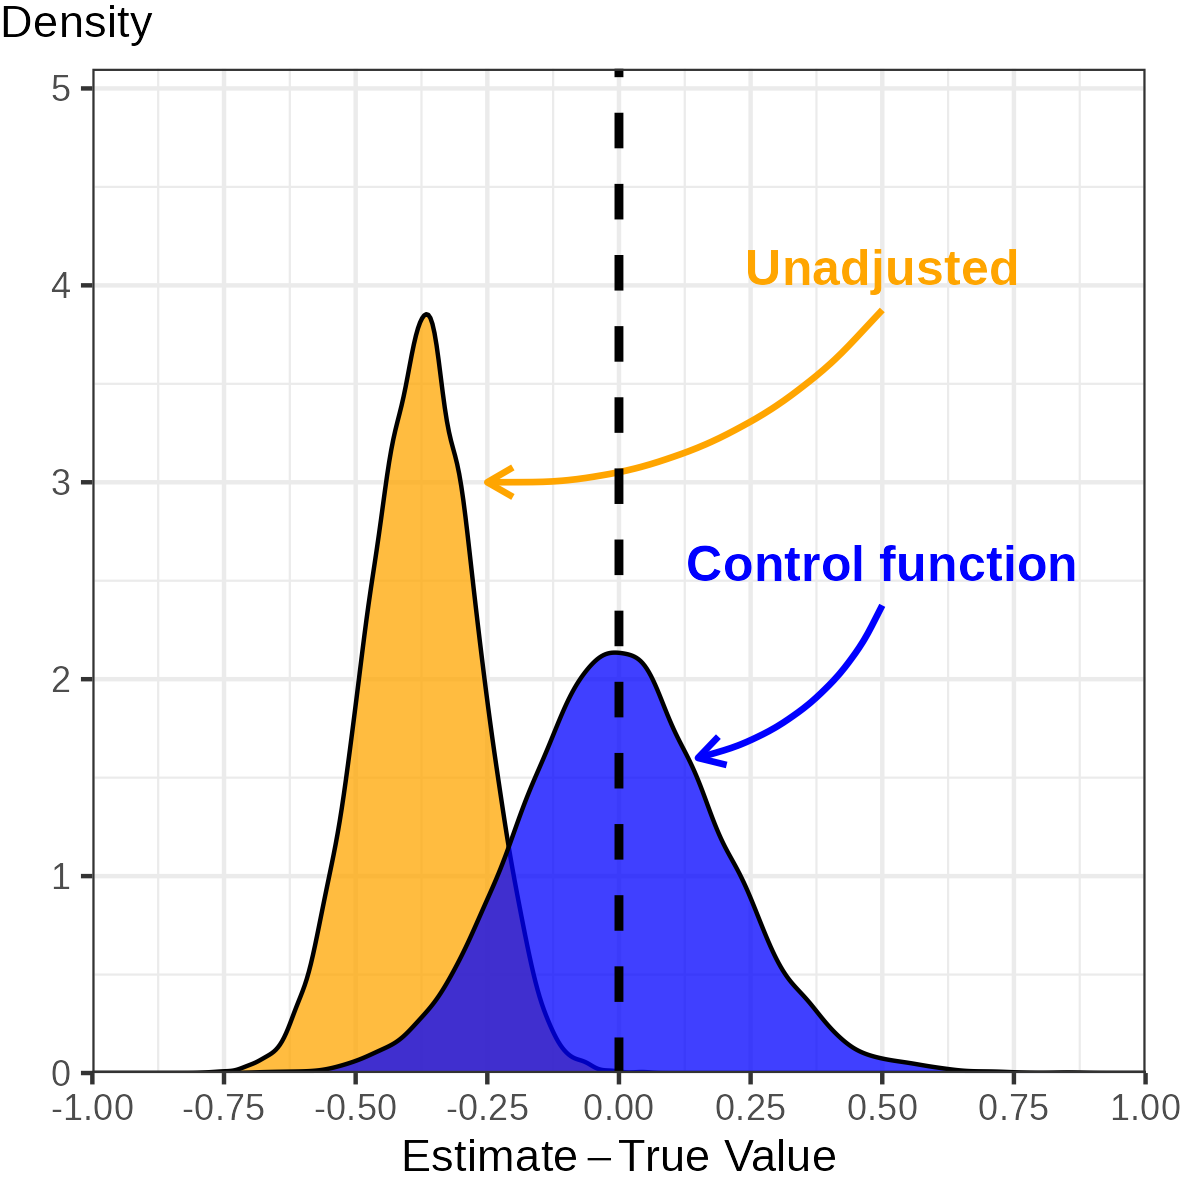
\includegraphics[width=\textwidth]{
            ../programs/simulations/sim-output/heckit-direct-dist.png}
    \end{subfigure}
    \begin{subfigure}[c]{0.475\textwidth}
        \centering
        \caption{AIE.}
        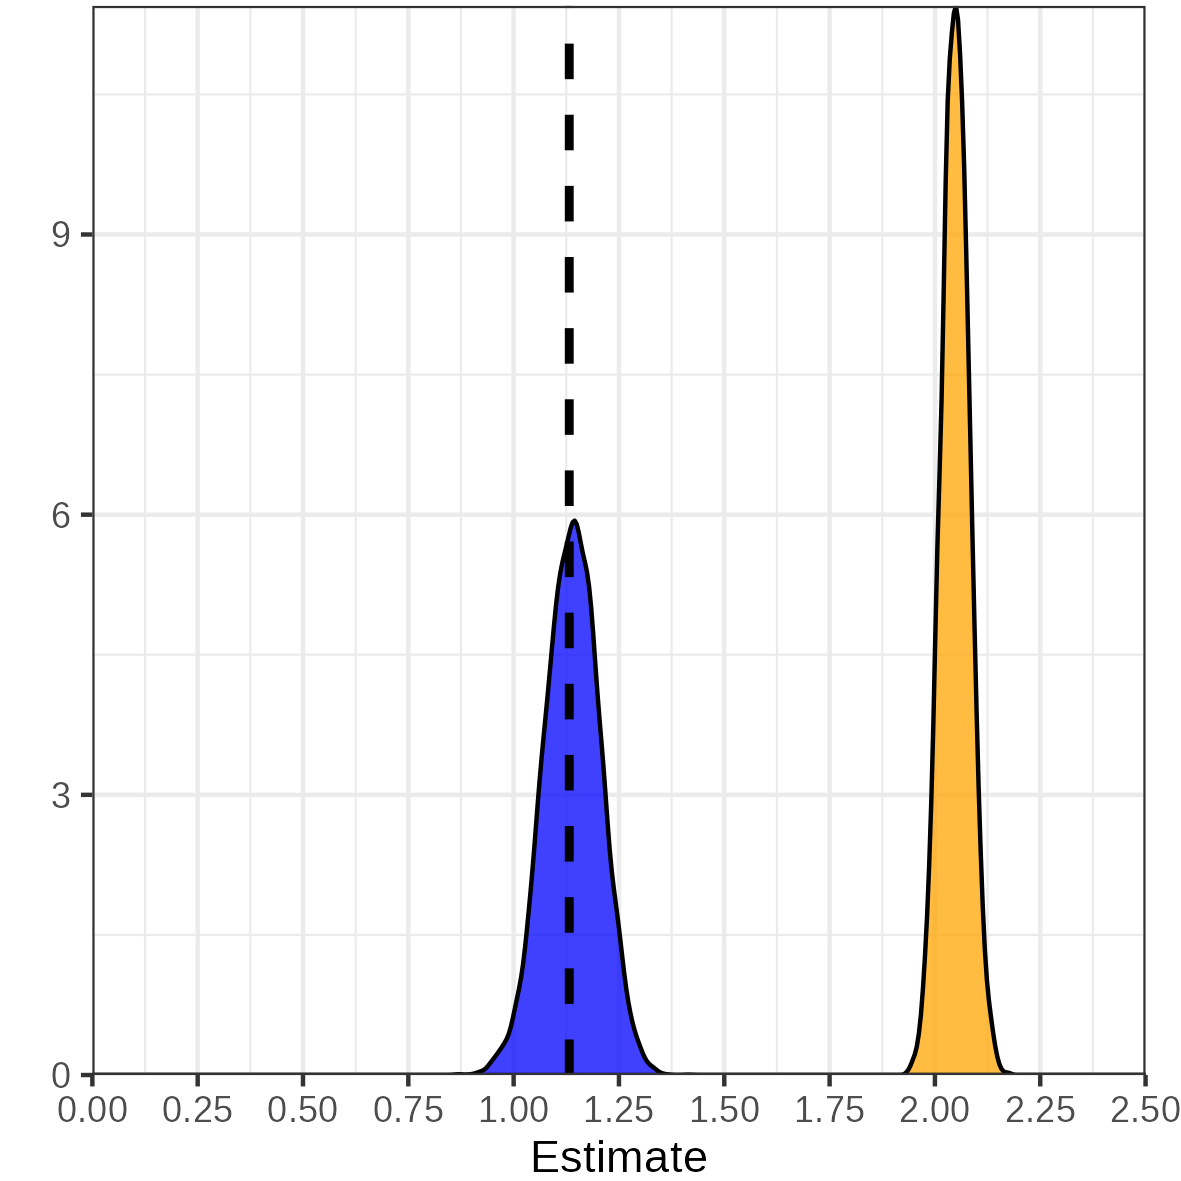
\includegraphics[width=\textwidth]{
            ../programs/simulations/sim-output/heckit-indirect-dist.png}
    \end{subfigure}
    \label{fig:cm-heckit-dist}
    \justify
    \footnotesize    
    \textbf{Note:}
    These figures show the empirical density of point estimates, for 10,000 different datasets generated from a Roy model with correlated normally distributed error terms (further described in \autoref{sec:controlfun}).
    The black dashed line is the true value;
    orange is the distribution of conventional CM estimates,
    and blue estimates with a Heckman selection adjustment.
\end{figure}
